\chapter{系统设计与实现}
\section{预期目标}
image computation指的是通过当前系统状态与转移关系,计算下一步系统状态。
在模型检测中,image computation是关键的一步。
过去传统模型检测已发展出多种高效的计算算法,特别是利用二叉决策图(BDDs)符号性表示初始状态和转移关系,以及利用状态空间划分和电路划分加速图像计算过程。然而,量子系统的模型检测尚处于起步阶段。
本次研究的重要目标就是利用TDD,构建量子系统的image computation,从而为未来的工作奠定基础。

考虑到量子计算的特殊性,可以利用一系列的优化策略,主要包括基于张量网络的结构特性和TDD的有效性能。通过这些优化,可以提升量子图像计算的效率,尤其是在处理复杂量子系统时的性能表现。

\section{研究方法}
本次研究的主要目的是借助TDD数据结构,构建能快速计算量子模型检测中可达问题的方案。本次研究的主要挑战在于尽可能减少程序的运行时间以及空间资源。为此,需要采用一系列方法来开发更有效的算法,以优化TDD操作和收缩张量网络。其中包括开发新技术来分割张量网络和优化TDD结构。
下面简单介绍以下具体研究方法。

\begin{myen}

\item \label{addition}关于常用的量子线路划分方法,
第一种被称为addition\citep{chen2018classical}。将量子电路视为张量网络,首先将一个量子电路C转换成无向图G。G中的每个节点表示量子电路的一个索引,并且如果它们是相同门的输入或输出索引,则在G中连接两个节点。并且当满足以下两个条件之一时输入和输出索引不变:
\begin{itemize}
	\item 是对角线量子门的输入和输出索引;
	\item 是受控门的控制比特位的输入和输出索引。
\end{itemize}
	
图\ref{fig:addition}展示了Grover\_3电路图的索引链接图。该图描述了量子电路的连通性,通过选择图中连通度最大的索引可以对电路进行分割。因此选择图中连通度较大的$x_1^1,x_1^3x_2^1$可以对电路进行较好的划分。
 
\begin{figure}[!htbp]
	\centering
	\includegraphics[height=6cm]{Img/cir_index_graph.pdf}
	\caption{Grover\_3的索引连接图}
	\label{fig:addition}
\end{figure} 

\item 另一种常用的电路划分方法成为contraction。在这一方法中,将量子电路划分为若干个较小的部分,其收缩等于原始电路。对于两个预设整数参数k1和k2,将电路划分为若干小电路。其中每个小电路涉及最多k1个量子比特,并且与至多跨越不同部件的k2个多比特门相连。图\ref{fig:contraction}展示了对Bit flip电路进行k1=3,k2=2的拆分结果。
\begin{figure}[!htbp]
	\centering
	\includegraphics[height=7cm]{Img/cir_contraction.pdf}
	\caption{对Bit flip电路进行contraction的拆分}
	\label{fig:contraction}
\end{figure} 


\item \label{contraction}在BDD中,索引的顺序很重要。因为索引顺序会直接影响BDD的大小。一个良好的变量顺序可以使得BDD比一个糟糕的变量顺序小得多。图\ref{fig:bdd-compare}的了两张图都表示了布尔函数ƒ(x1,...,x8)=x1x2+x3x4+x5x6+x7x8,但图\ref{fig:bdd-good}的结构更简单。其中图\ref{fig:bdd-bad}的索引顺序为\{x1,x3,x5,x7,x2,x4,x6,x8\},图\ref{fig:bdd-good}的索引顺序为\{x1,x2,x3,x4,x5,x6,x7,x8\}。找到一个好的索引顺序是一个NP问题。在工程实现中,目前只能通过小规模电路上寻求规律,然后在更大规模电路中应用较优顺序。

\begin{figure}[!htbp]
	\centering
	\begin{subfigure}[b]{.4\textwidth}
        \centering
        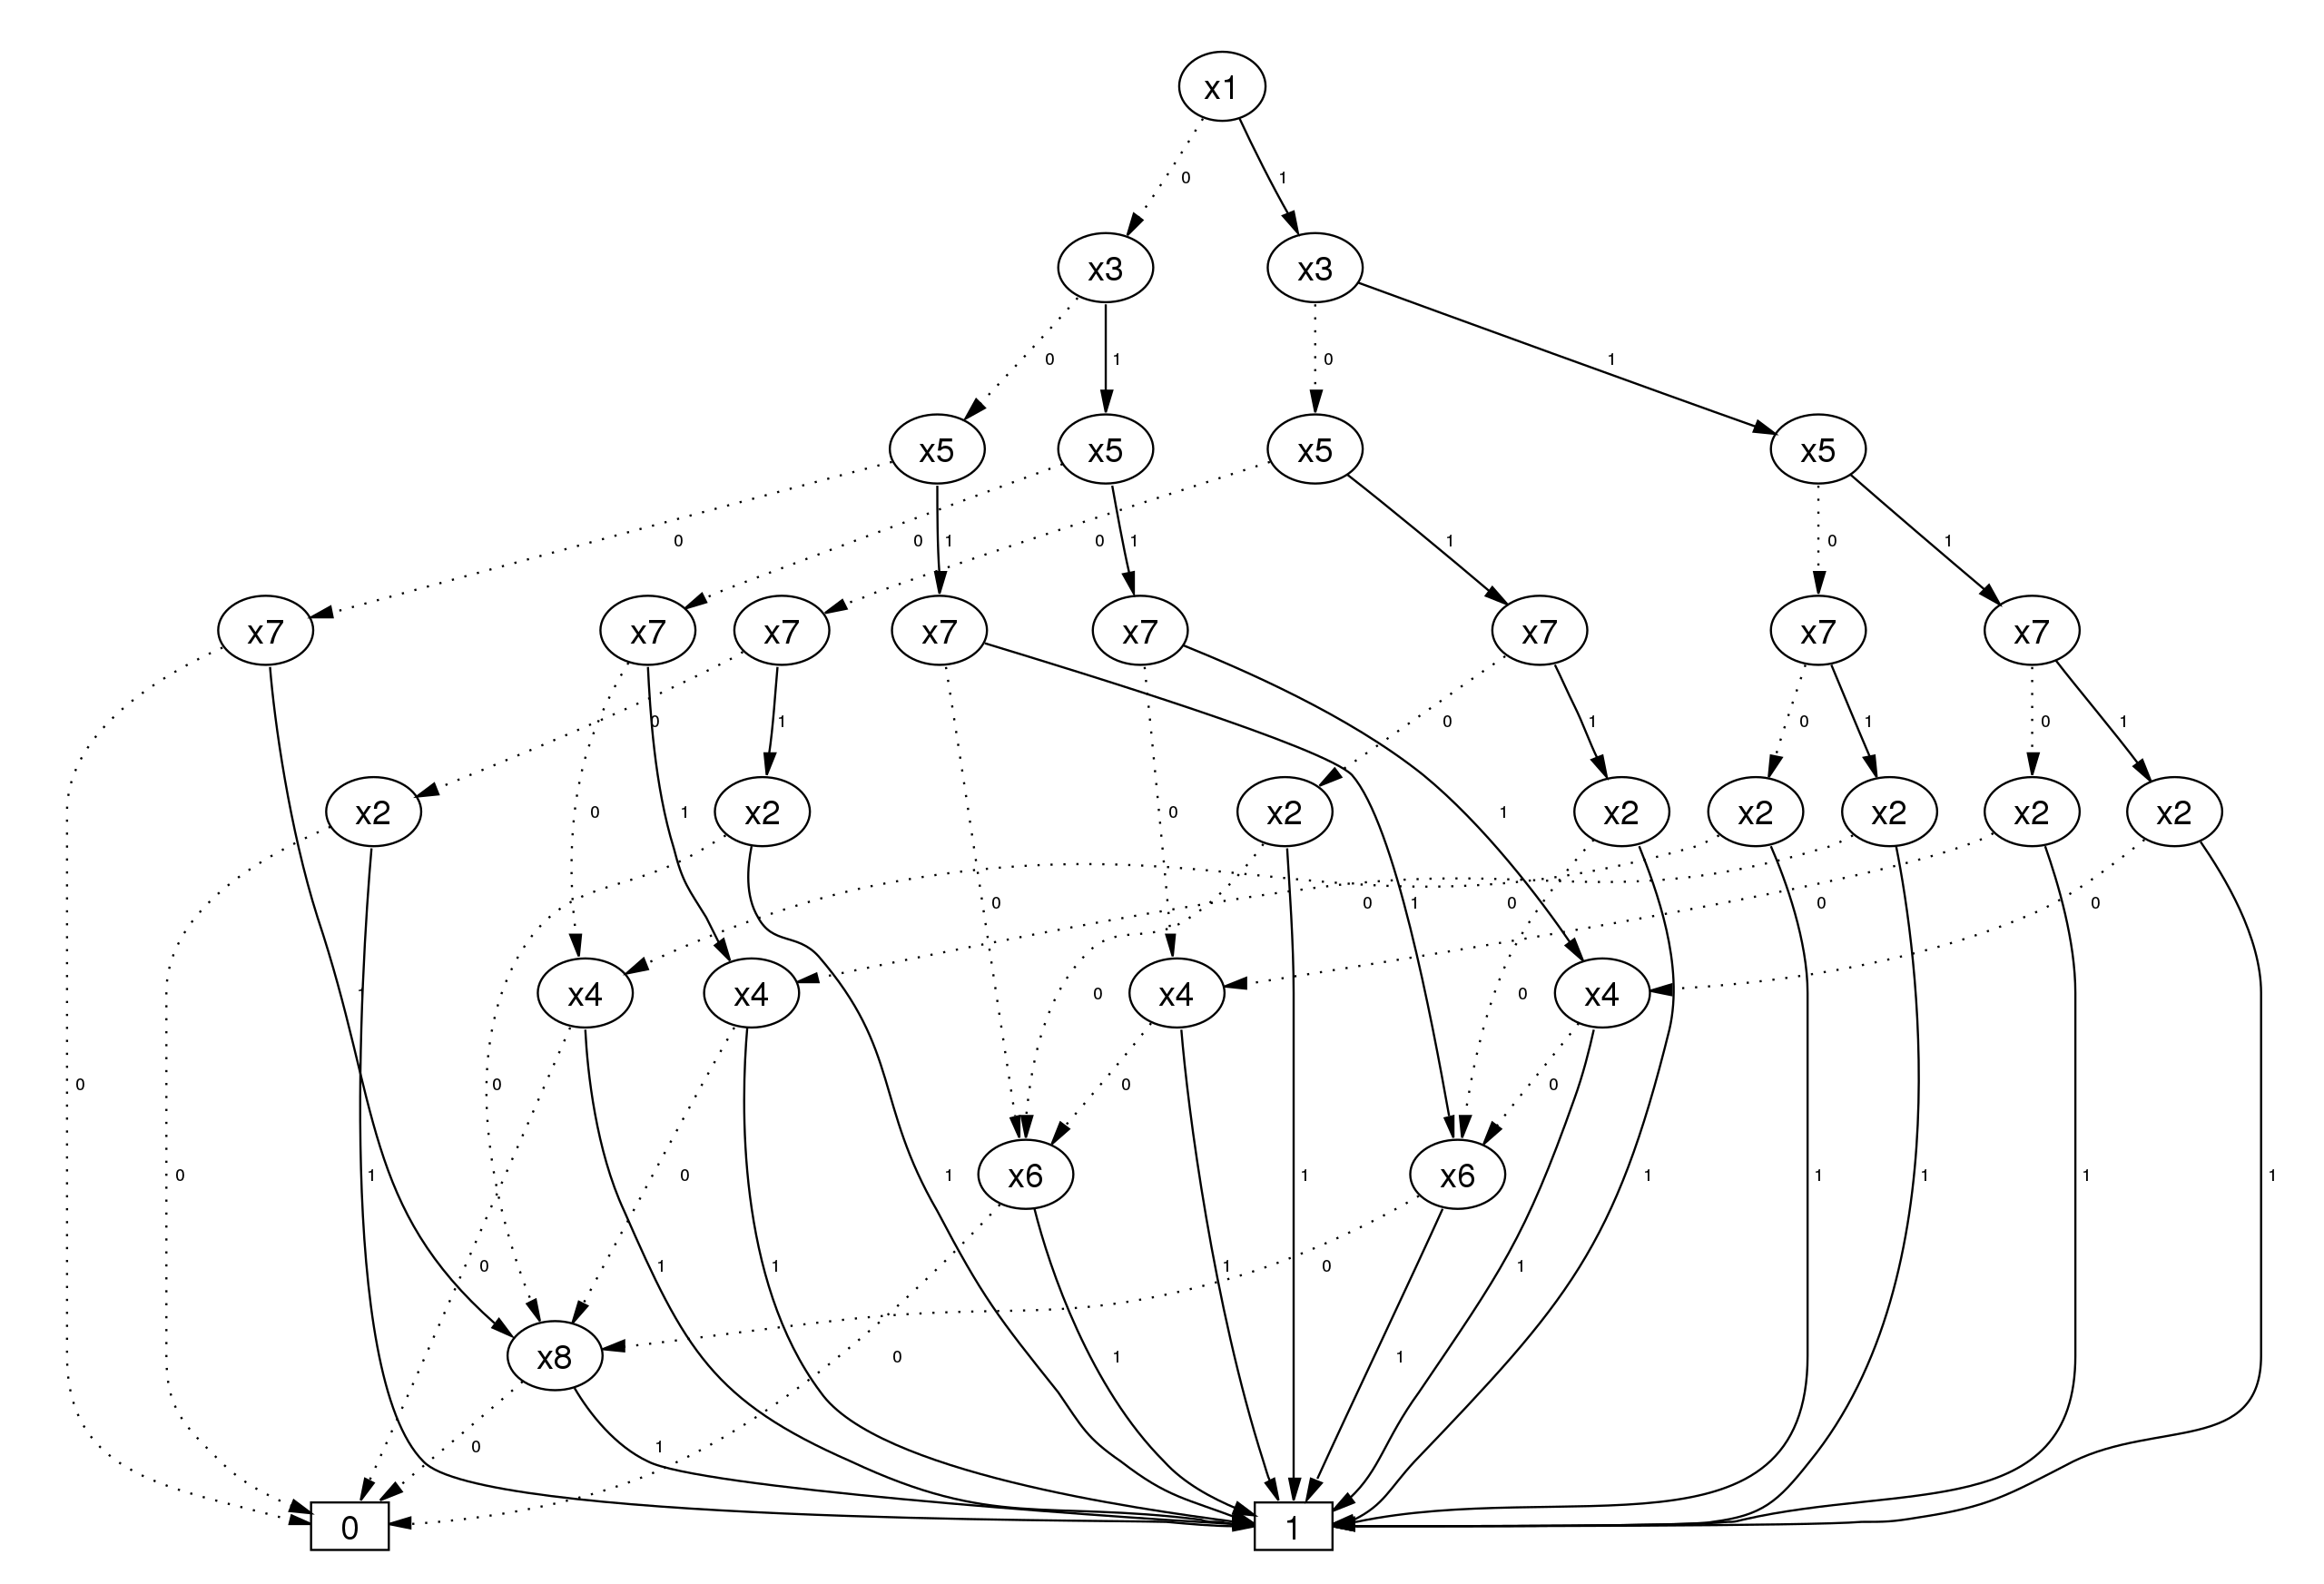
\includegraphics[height=6cm]{Img/BDD_Variable_Ordering_Bad.svg.pdf}
		\caption{索引顺序为\{x1,x3,x5,x7,x2,x4,x6,x8\}}
		\label{fig:bdd-bad}
	\end{subfigure}
    \qquad
	\begin{subfigure}[b]{.4\textwidth}
        \centering
        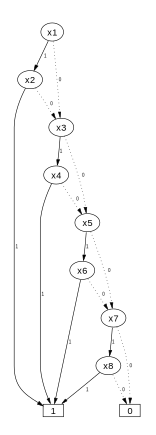
\includegraphics[height=6cm]{Img/BDD_Variable_Ordering_Good.svg.pdf}
		\caption{索引顺序为\{x1,x2,x3,x4,x5,x6,x7,x8\}}
		\label{fig:bdd-good}
	\end{subfigure}
	\caption{同一布尔函数在不同索引顺序下的结构图\citep{wiki:bdd}}
	\label{fig:bdd-compare}
\end{figure}


\item 由于量子状态都在同一希尔伯特空间中。因此作用某些算子后,不同的量子状态可能等价。
当存储算子的资源少于存储状态的资源时,就有可能存储算子表示不同的状态\citep{vinkhuijzen2023limdd}。图\ref{fig:qmdd-example}表示了一个QMDD的例子,应用等价性,可以化简为图\ref{fig:limdd-example}。
TDD也可以应用类似技术,进行进一步化简,从而降低资源要求。
\begin{figure}[!htbp]
    \centering
    \begin{subfigure}[b]{.4\textwidth}
        \centering
        \includegraphics[height=8cm]{Img/limdd.pdf}
        \caption{一个QMDD示例}
        \label{fig:qmdd-example}
    \end{subfigure}
    \begin{subfigure}[b]{.4\textwidth}
        \centering
        \includegraphics[height=8cm]{Img/limdd_reduce.pdf}
        \caption{应用等价性化简图\ref{fig:qmdd-example}}
        \label{fig:limdd-example}
    \end{subfigure}
\end{figure}
\end{myen}
\section{软件系统实现}
为了实现软件的高效运行,模块化设计至关重要。
每个模块在软件系统中扮演着关键角色,并且具有特定的功能和目的。以下是本次毕业设计中软件必须包含的模块及其重要性的说明:

\begin{itemize}
    \item \textbf{输入处理模块}:该模块的主要职责是处理输入数据,例如接收用OpenQASM格式编写的量子算法代码。其核心功能是将这些代码转换为TDD表示形式。鉴于当前存在多种量子编程语言,此模块的模块化处理能够显著提升系统的灵活性和兼容性。
    \item \textbf{内存管理模块}:本模块负责管理TDD节点的存储和维护。当创建新的TDD节点时,它会运用哈希算法与现有节点进行对比,以避免重复创建相同节点。这种方法不仅减少了内存占用,还提高了处理效率。
    \item \textbf{TDD基础模块}:该模块主要执行TDD节点的压缩操作,或者导出TDD的树状结构图。节点收缩是TDD核心的运算过程,而树状结构图的导出功能则有助于用户更好地理解和分析TDD的结构。
    \item \textbf{TDD算法模块}:此模块为TDD提供更复杂的算法支持。例如,它能够调整节点收缩的顺序,以优化系统运行效率。此外,它还能执行其他高级功能,如检验TDD是否存在于特定子空间中。
\end{itemize}

